\documentclass[titlepage]{article}
\usepackage[T1]{fontenc}
\usepackage[utf8]{inputenc}
\usepackage{biblatex}
\usepackage{titling, lipsum}
\usepackage{graphicx}
\usepackage{indentfirst}
\usepackage{geometry}
\usepackage{hyperref} 
\usepackage{float}

\graphicspath{{./images/}}

\geometry{
 a4paper,
 total={170mm,257mm},
 margin=1in
}

\addbibresource{bibliography.bib}

\begin{document}
\begin{titlepage}
	{\centering
	{\scshape\huge Comparison of SLAM methods with CUDA implementation \par}
	\vspace{1cm}
	{\scshape\Large Course: Research project - GPU algorithms \par}}
	
	\vspace{1cm}
	\noindent\textbf{Coordinator}: Krzysztof Kaczmarski\\
	\textbf{Authors}: Michał Rogala, Szymon Stasiak, Mateusz Śliwakowski\\
	\textbf{Description}: Short description\\
	\textbf{Code repository}: \href{https://github.com/Sliwson/cuda-slam}{https://github.com/Sliwson/cuda-slam}\\
	\textbf{Code license}: MIT\\
	\textbf{Input files}: Point clouds as .obj files\\

	\vfill
	{\large \today \par}
\end{titlepage}

\tableofcontents
\newpage

\section{Report goals}
%What we will know after reading this document?

The report is devoted to a research of SLAM methods using CUDA technology. We want to give a brief introduction what SLAM is and what are its applications. After reading the document you should know three different methods of approaching the problem, their advantages and disadvantages. The cornerstone of the work is answering the question - how well these methods can be converted to GPU architecture and how much will we gain?

\section{Problem statement}
%Description of the problem, motivating example, killer application, etc.

\subsection{Theoretical background}
\textbf{Simultaneous localization and mapping} (in short SLAM) is the computational problem of constructing or updating a map of an unknown environment while simultaneously keeping track of an agent's location within it \cite{ms-wiki1}. In theory the problem can be simplified to more mathematical definition - given two point sets $P_1 = \{x_1,\dots, x_n\}$ and $P_2=\{y_1, \dots, y_n\}$ find translation $t$ and rotation $R$ that minimizes the Mean Square Error:
$$MSE(R, t) = \frac{1}{N}\sum_{i=1}{N}(x_i - Ry_i - t)^2$$

The reality, unfortunately, is much more complicated. Sizes of point sets might differ, clouds are unordered and noise points can occur.

\subsection{Applications}
The main field of SLAM application is robotics. There are a lot of machines that utilizes this algorithm to keep track of the space in which they are moving. The most popular are autonomous vacuum cleaners such as presented below.

\begin{figure}[H]
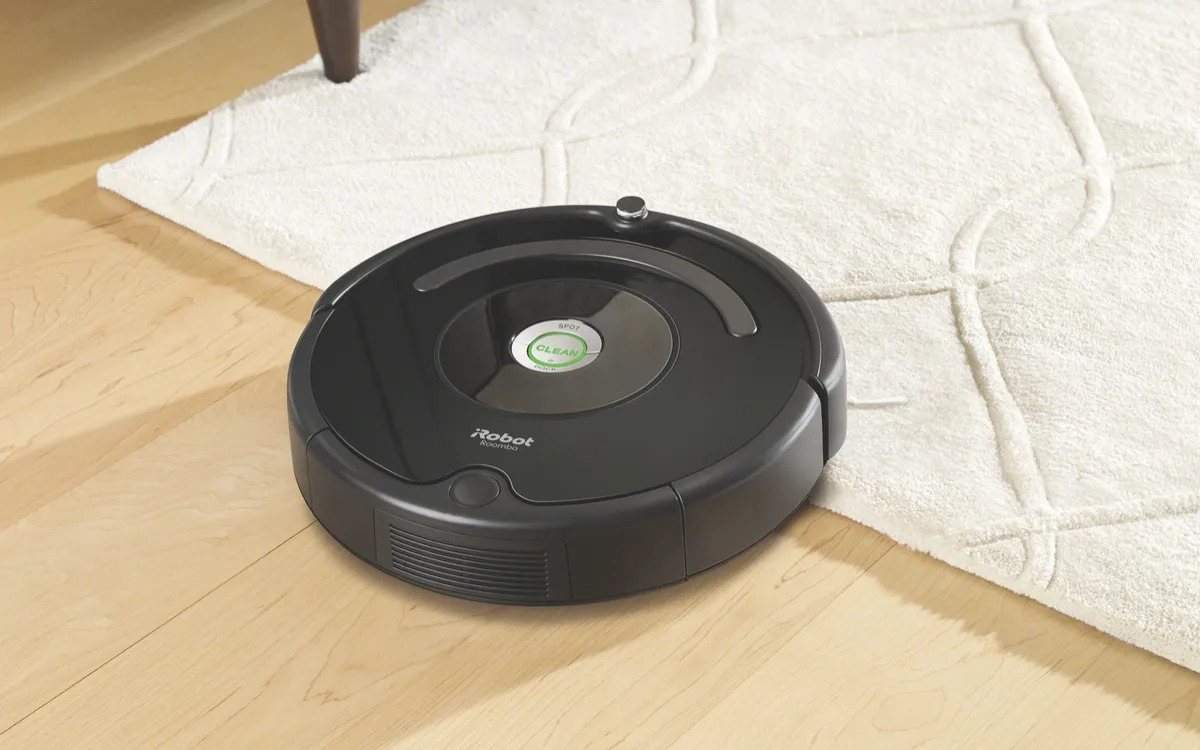
\includegraphics[width=\textwidth]{ms-img1.png}
\caption{Autonomous vacuum cleaner}
\end{figure}

Another popular application is mapping real life environments to digital equivalents. The programs produce \textit{Geospatial mappings} which can be later processed and analysed. Variety of different devices is used such as hand scanners, drone scanners or even satellites. Due to rapid technological progress nowadays, even smartphone cameras can be used to perform simple environmental scan.

\begin{figure}[H]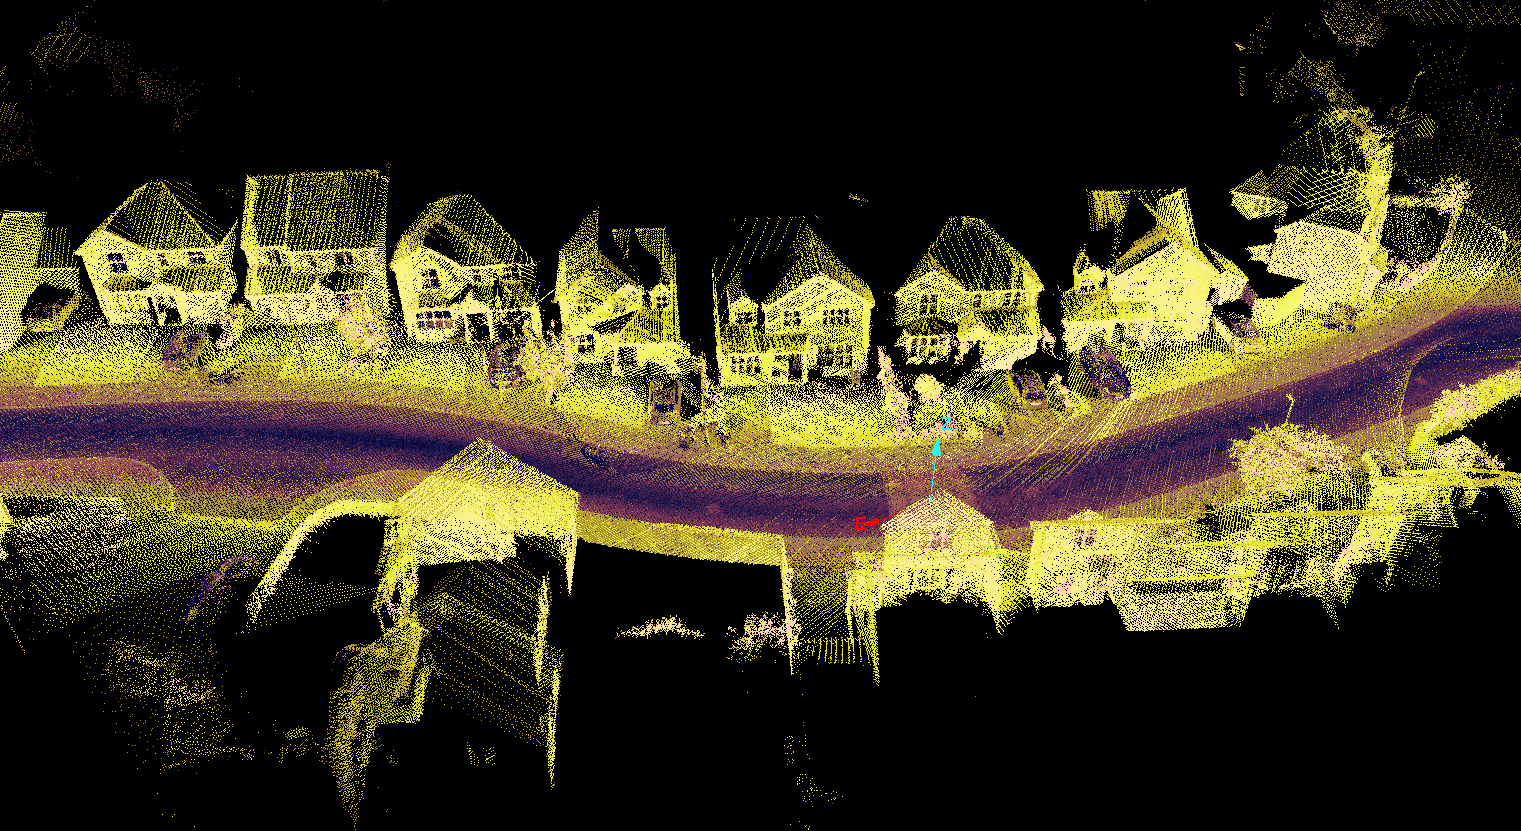
\includegraphics[width=\textwidth]{ms-img2.jpg}
\caption{3D laser scan}
\end{figure}

\section{Computational method}
The most important ideas in the algorithm necessary to understand how it works.
Are there any differences from other methods?
Are there any novel ideas?
\section{Program architecture}
Short description on the modules of the system, requirements, dependencies, etc.
\section{Input data description}
File formats, api used to read, dependencies, data sources, etc.
Is there any institution providing the input data?
References to public databases.
\section{Execution, configuration and user guide}
How can one replicate the experiments?
Any relevant information and runtime howtos.
\section{Description of the results}
Performance of the system for different input data/parameters.
How we understand the results and why are they correct?
Can we formulate any conclusions from the experiments?
\section{Remarks}
Any remarks to the results and methods.
\section{Future works}
What do we want to do in future, improvements.

This is bibliography sample - it was noted in\cite{ms-paper1}.

\newpage
\printbibliography

\end{document}

